\section{Path Joining}

\begin{figure*}[ht]
\centering
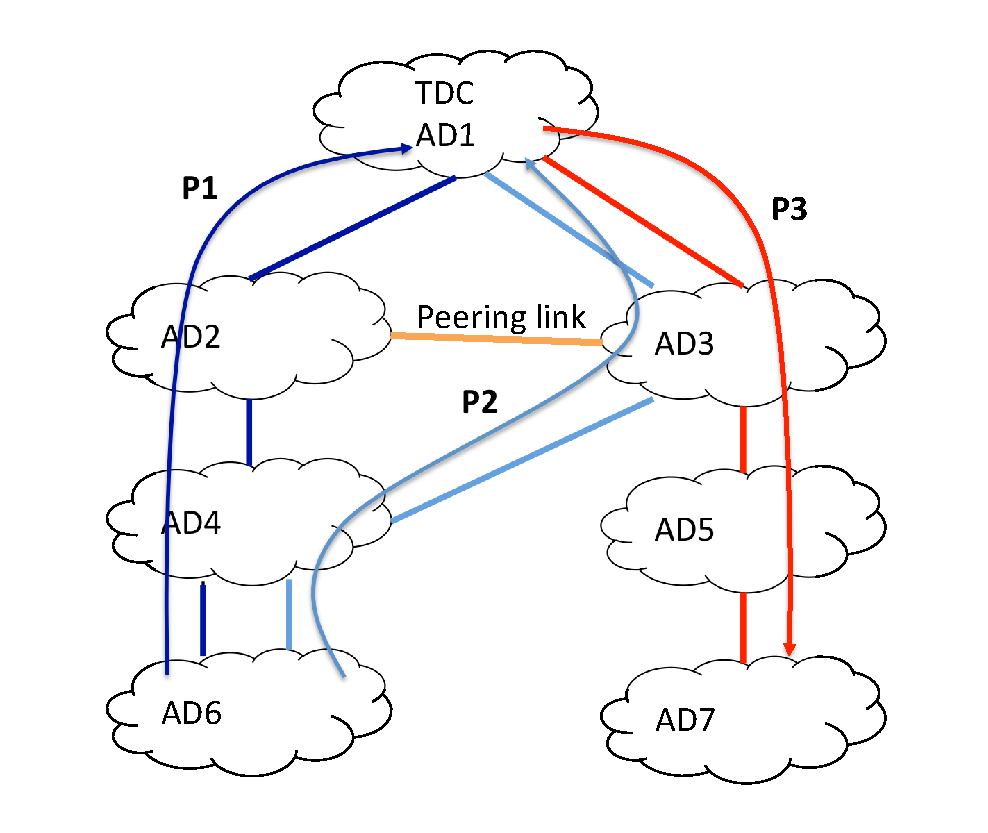
\includegraphics[width=.7\columnwidth]{./fig/pathjoin.eps}
\caption{Example: Path Joining.}~\label{fig:pathjoin}
\end{figure*}

\begin{figure*}[ht]
\centering
\mbox{\subfigure[Up-path Table]{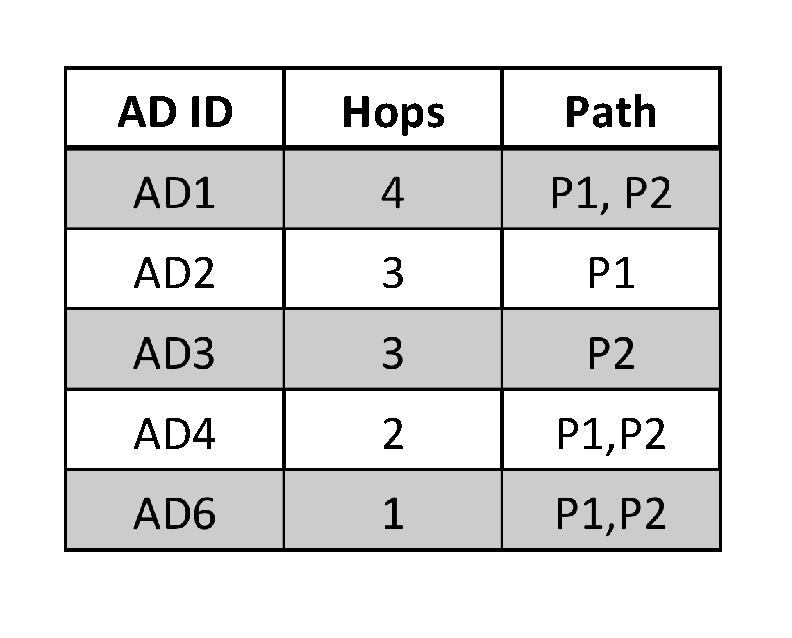
\includegraphics[scale=.5]{./fig/uppath_table.eps}}~\label{fig:uppath-table}\quad
\subfigure[Down-path Table]{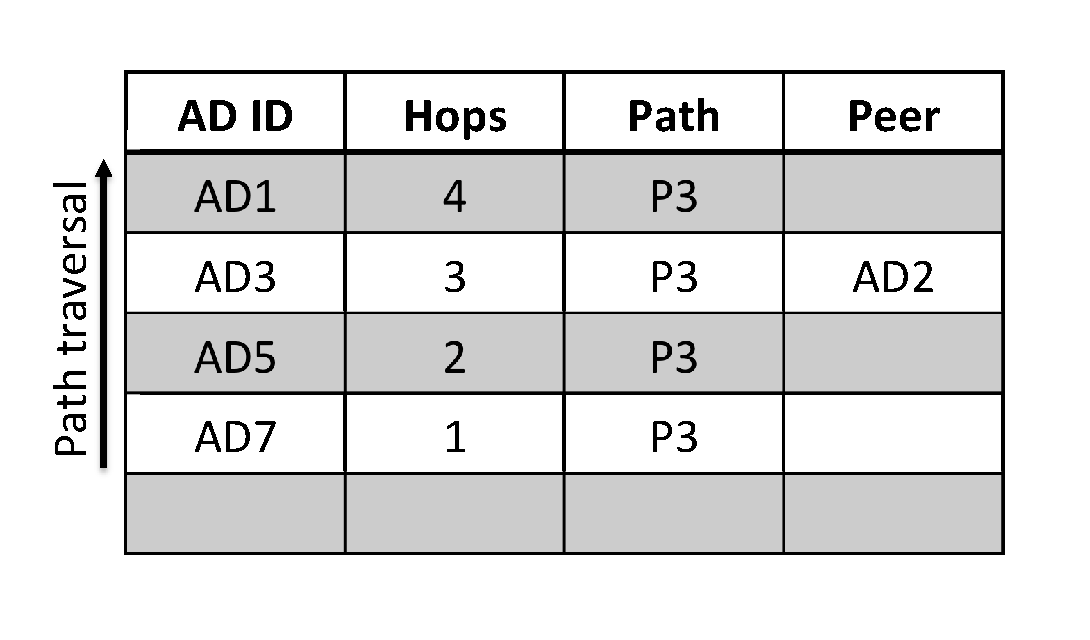
\includegraphics[scale=.5]{./fig/downpath_table.eps}}~\label{fig:downpath-table}}
\caption{Example: The up-path and the down-path tables for two up-paths (i.e., P1, P2) and a single down-path (P3) for Figure~\ref{fig:pathjoin}.}
\end{figure*}

In this section, we describe how to construct an end-to-end path using the up-paths and down-paths provided by the local \PS.

The local \PS has a large number of up-paths provided by the local \BS and a set of down-paths to a specific destination \AD provided by a \TDC \PS.
An end-to-end path is constructed by joining an up-path and a down-path and is represented by a series of opaque fields preceded by SCION common header and two special opaque fields (i.e., up and down timestamps). Path joining can be performed either by the local \PS or by a client who wants to contruct a path. Path joining at a client is very simple as the client join all possible combination of up- and down-paths and select the best path among them. However, such brute-force joining is very inefficient if it is performed at the local \PS because (1) the \PS has a large number of up-paths and possibly many down-paths (if the \PS caches the down-paths of an \AD and reuse them until they expire, instead of using them once) and (2) each path may contain many peering links. In this case, joining all up- and down-paths incurs a huge overhead to the \PS. We resolve this issue by designing an efficent path joining algorithm below.

A half-path (either up- or down-path) consists of a series of ADs, where each AD is identified by its ADID and its ingress and egress interfaces. Hence, even if two paths contain the same series of ADs, they can differ if any one of the interface is not same. However, we do not distinguish a path by its timestamps.

Our algorithm finds a shortest path(s) in terms of \AD hops and consists of three parts, which are up-path table construction, down-path table construction, and path traversal.

\subsection{Up-path Table}
The up-path table consists of three field as Figure~\ref{fig:uppath-table}: ADID, Hops, and Path. ADID is the AD identifier, Hops is the distance from the endpoint AD, and Path is the pointer to the path (i.e., PCB) that contains the current ADID. Each field is identified by a unique ADID, hence if a path contains a unique AD, it creates a new entry. If an ADID already exsits in the table, there are three choices: (1) if the Hops of the current path is same as the one in the table, its pointer is added to the Path field; (2) if the Hops is less than the existing one, it replaces the current one; and (3) if the Hops is greater than the existing one, it is discarded. For example, in Figure~\ref{fig:pathjoin}, P1 consists of AD1,AD2,AD4, and AD6 and is filled into the up-path table in the reverse order of PCB propagation. P2 is added to the table in the same way, yet only AD3 creates a new entry since other ADs already exist in the table (hence P2 is added to the Path field of existing AD entry).

\subsection{Down-path Table}
The down-path table has another field, peer ADID, in addition to all fields in the up-path table. The peer ADID is used to construct an end-to-end path through a peering link. Since the relationship of a peering link is symmetric (i.e., if it appears the up-path, it should appear in the down-path, and vice versa), we only need to add this information either to the up-path table or to the down-path talbe. We add the peering information to the down-path table since the number of down-paths is smaller than that of up-paths, and the path construction starts from the down-path (hence it is more efficient to include it in the down-path table).

\subsection{Path Traversal}
With the up-path and the down-path tables, one can construct an end-to-end shortest path as follows.
\begin{enumerate}
\item Start from the endpoint \AD in the down-path table.
\item Find the same ADID staring from the endpoint (i.e., Hops == 1) \AD toward TDC \AD in the up-path table.
\item If the same ADID exists in the ADID field of the up-path table, the corresponding AD is the crossver \AD through which a shortcut path is constructed.
\item If the path-length of the shortcut path is less than the current minimum, replace the shortest-path list with the shortcut path.
\item If the path-legnth of the shortcut path is equal to the current minimum, add the shortcut path to the shortest-path list.
\item For each peer ADID in the current down-path entry, do 2-5 with the peer ADID. If a matching ADID is found in the up-path table, a shorcut path is constructed through a peering link between the ADID and the peer ADID.
\item Repeat 2 - 6 for all \ADs toward TDC \AD in the down-path table. 
\end{enumerate}

We note that an end-to-end path consists of a pair of up-path and down-path, hence is stored as a pair. We also note that if the Path field at the crossover \AD has multiple entries (e.g., up-path P1, and down-paths P2, P3), both paths are added to the shortest-path table (i.e., (P1,P2), (P1,P3)). We can set the maximum size of the shortest-path list (e.g., to $k$) and store the (first) k-shortest paths in order not to keep unnecessarily many paths.


\begin{comment}
Our solution is AD-level (turning point) search plus opaque-field path construction. The reason for this approach is as below. First, we should be aware that we are dealing three data structures at the same time -- path, AD and opaque-field. Each path contains several ADs and each AD on the path is represented by an opaque-field with ingress interface, egress interface and MAC. For a single AD, there may be several paths that cross it so it could map to more than one opaque-field. To increase algorithm efficiency in finding the turning point for shortest path search, we need to extract the most relevant information from the path-AD-OF data and hide irrelevant details. That is the idea of AD-level search. In this stage we only care about finding the AD-level turning point and we hope that we can construct the end-to-end path from this turning point. 
To support the idea of AD-level search, we designed a data structure called âœAD table❠as the up-path AD table example shows below.

AD6 is the source, AD7 is the destination and AD1 is the TD core. Each entry corresponds to an AD on the path with a vector of pointers to the path it belongs. For shortest path search we only store the pointer of the path whose AD is closest to the source. For instance, letâ™s assume there is another path3 that is AD6-AD9-AD4-AD2-AD1. Only p3 to path3 will be added to the AD6 and AD9â™s path vector because the hop numbers from AD4, AD2, AD1 to AD6 (source) are all larger than the current hops. 
	Similarly the AD table for down-path is as below.


	The only difference here is that there is another column called peer AD vector indicating to which ADs the entry AD has peering links. Not including peer AD vector in up-path AD table avoids information redundancy. It also helps save search time to put peer AD vector in the down-path AD table since there are less down-paths than up-paths.
		The AD-level search for turning point is to go through each entry of down-path AD table. First we see if the AD in the entry belongs to the up-path AD table, if so this AD is a cross-over point and we calculate the sum of hops of these two entries and compare it with the lowest path hop number, if it is less than we mark the entry ADs. Then we see if the peers of the AD belongs to the up-path AD table, if so there is a peering link then we calculate the total hops and compare and if it has less hop we mark the two ADs. In the case below, the AD3 in down-path table and up-path AD table is a crossover point that corresponds to the shortest path with 3+3-1=5 hops.

		Having found the âœturning pointâ, we pick one path pointer p3 in AD3â™s path pointer vector in down-path AD table and p2 in AD3â™s path pointer vector in up-path AD table to construct the full path (end-to-end path). This is called opaque-field-level path construction. The full path is shown as below.
\end{comment}
